\section{Results and Analysis}
\label{sec:results}

\subsection{Overall Scorecard}

Table~\ref{tab:scorecard} gives the final state of all six runs. The central empirical fact is simple: the PPO column directionally supports RAGEN's StarPO-S story, while the GRPO column reverses it.

\begin{table*}[t]
\centering
\small
\begin{tabular}{lllllll}
\toprule
\# & Run & Algorithm & Filter & Reward & Success & Format \\
\midrule
1 & PPO vanilla & PPO & 1.0 & \(-0.654\) & 0.000 & 0.000 \\
2 & PPO StarPO-S moderate & PPO & 0.5 & \(-0.185\) & 0.000 & 0.000 \\
3 & PPO StarPO-S aggressive & PPO & 0.25 & \(-0.060\) & 0.005 & 0.050 \\
4 & GRPO vanilla & GRPO & 1.0 & \(\mathbf{+0.225}\) & \(\mathbf{0.225}\) & \(\mathbf{0.808}\) \\
5 & GRPO filtered moderate & GRPO & 0.5 & \(-0.079\) & 0.005 & 0.369 \\
6 & GRPO filtered aggressive & GRPO & 0.25 & \(-0.072\) & 0.020 & 0.363 \\
\bottomrule
\end{tabular}
\caption{Final evaluation metrics at step 200. GRPO vanilla is the only run with sustained positive reward, non-trivial success, and high format compliance.}
\label{tab:scorecard}
\end{table*}

\begin{figure*}[t]
\centering
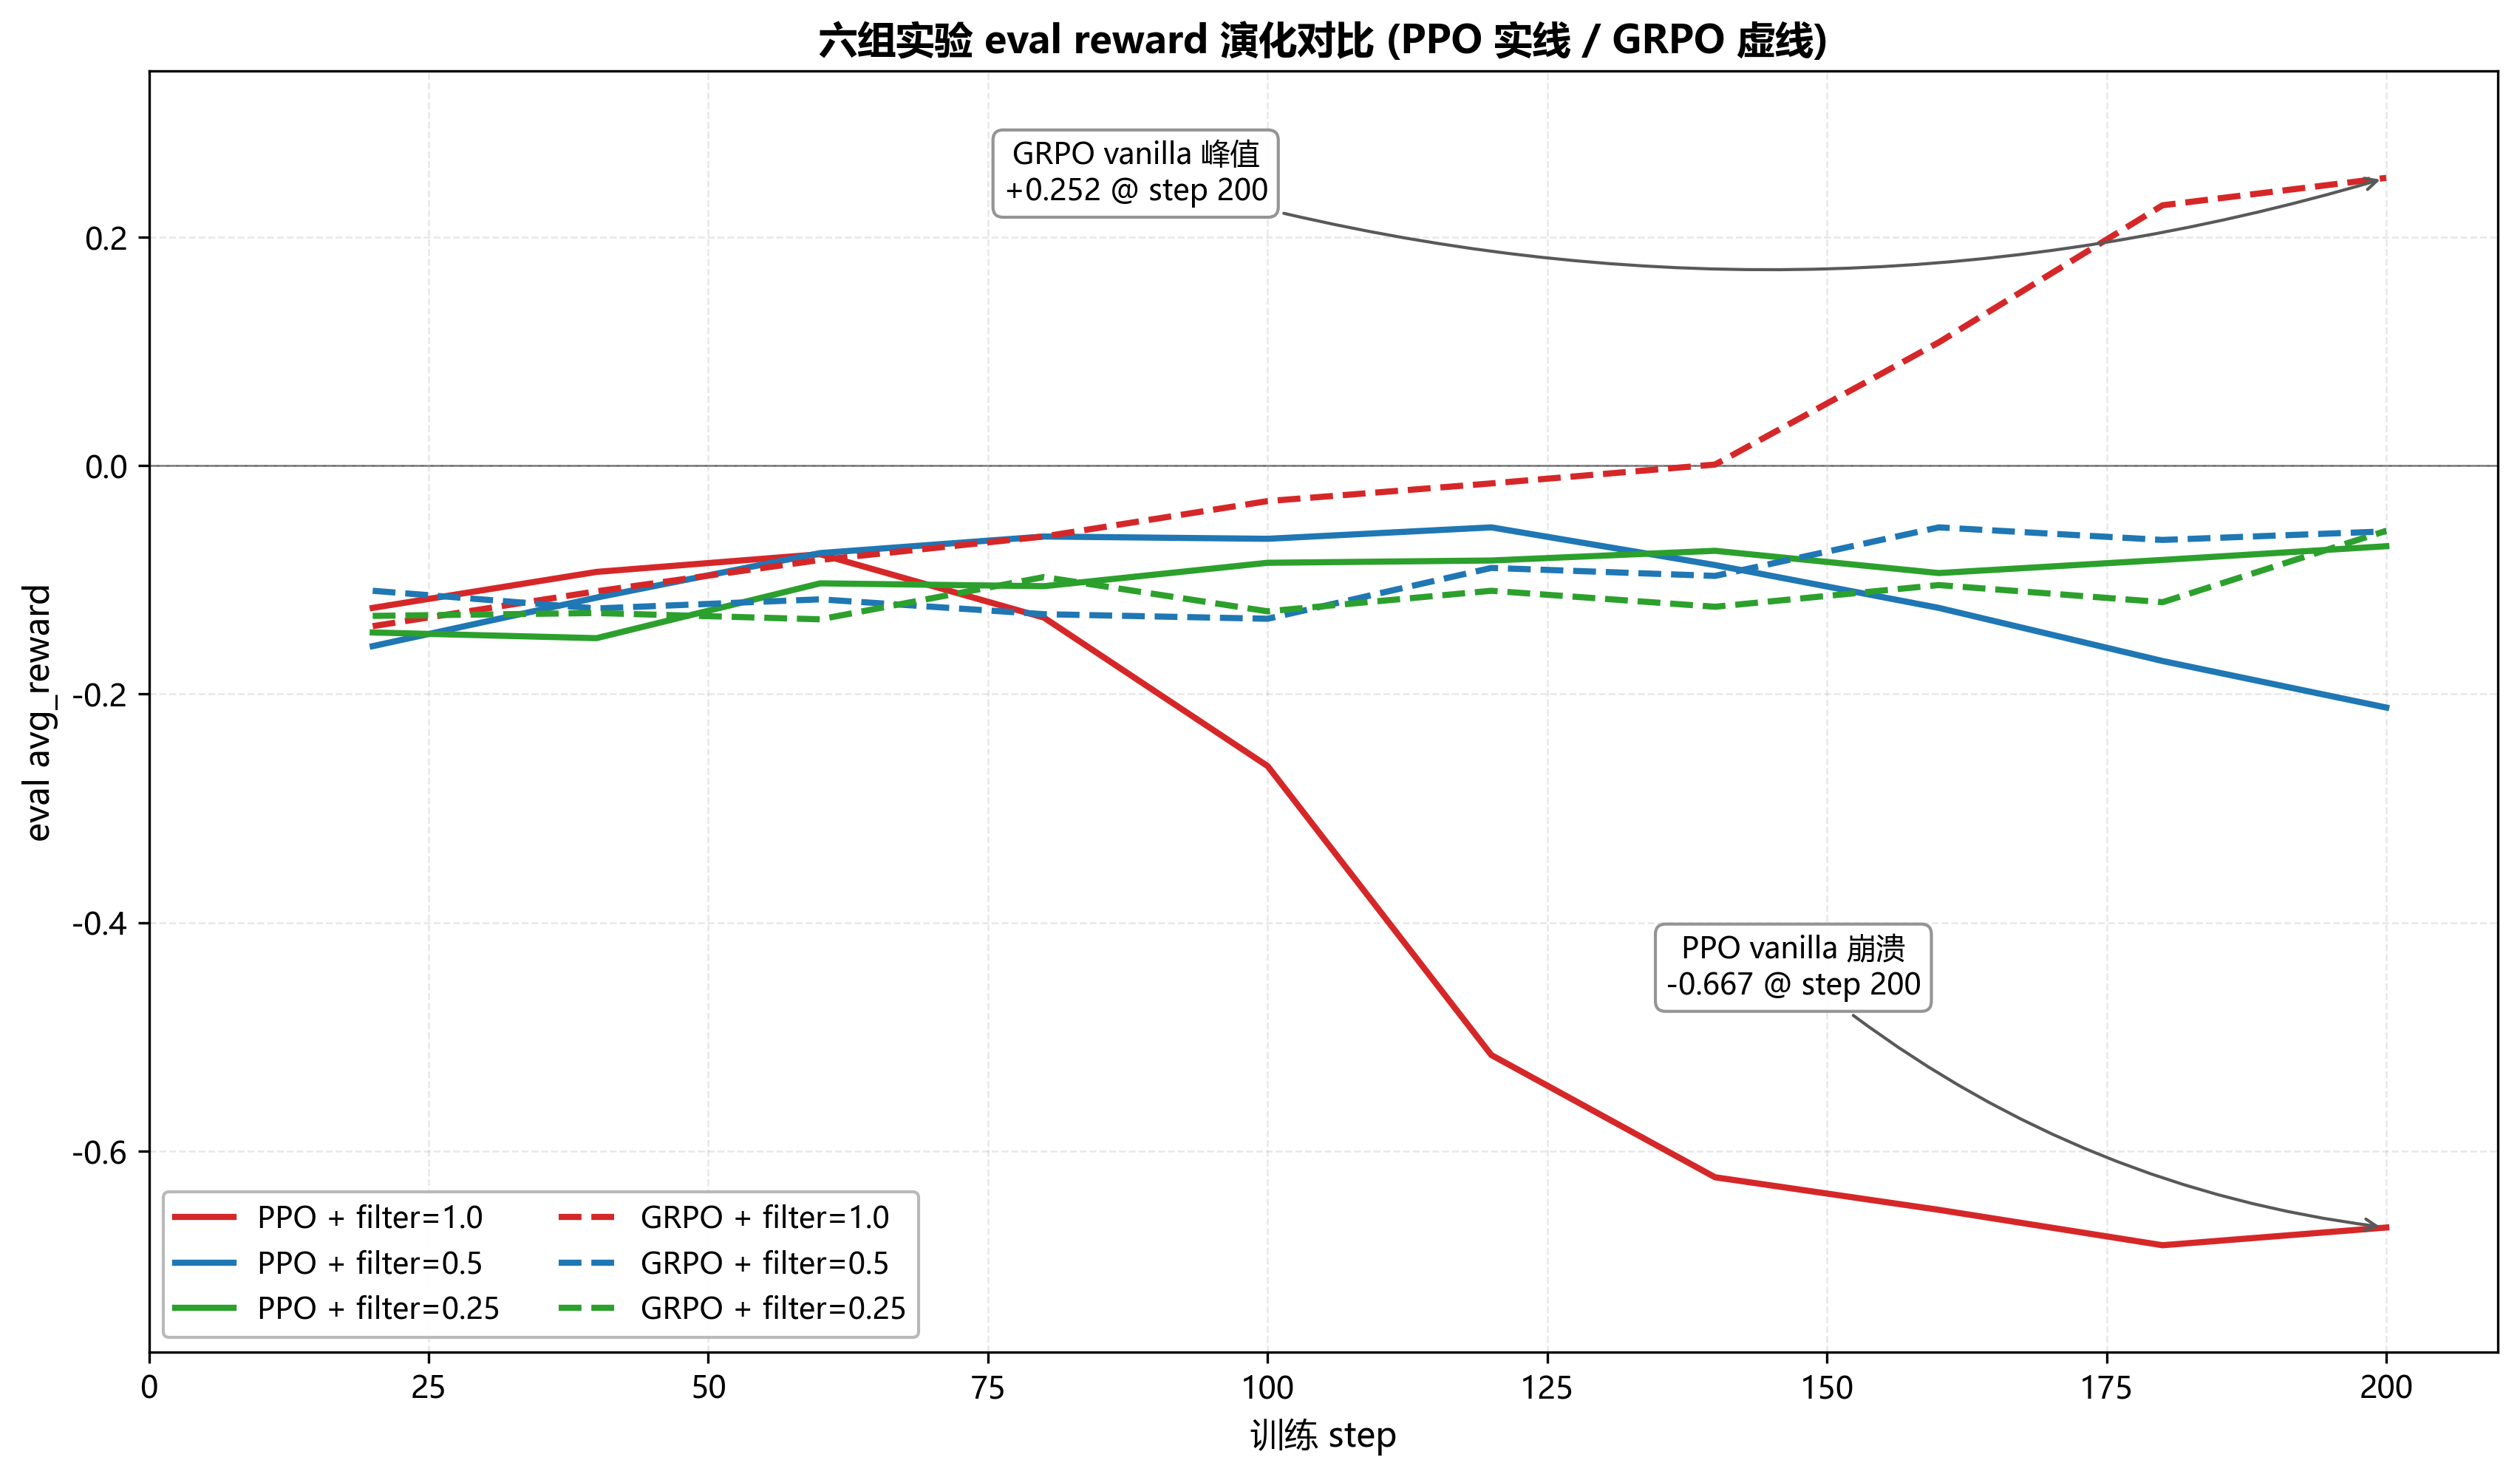
\includegraphics[width=\figw]{figures/fig01_eval_reward_6groups.png}
\caption{Evaluation reward over all six runs. PPO exhibits the expected filtering trade-off direction, while GRPO performs best with no variance filtering.}
\label{fig:reward}
\end{figure*}

Figure~\ref{fig:reward} shows the full reward trajectories. PPO with no filtering improves briefly and then collapses after step 100, ending at \(-0.654\). PPO with ratio 0.5 reaches its best point at step 120 and remains much better than vanilla at the end. PPO with ratio 0.25 is stable but nearly stagnant. GRPO behaves differently: vanilla GRPO steadily improves to \(+0.225\), while both filtered GRPO variants remain near the negative-reward plateau.

\subsection{PPO Directionally Reproduces RAGEN}

The PPO results support three RAGEN-style claims at the level of trend and mechanism.

\paragraph{P1: vanilla instability.}
PPO with filter ratio 1.0 deteriorates from \(-0.124\) at step 20 to \(-0.654\) at step 200, a roughly \(5.3\times\) worsening relative to the initial magnitude. This reproduces the instability direction in the RAGEN 0.5B sparse-reward setting.

\paragraph{P2: moderate filtering mitigates collapse.}
PPO with ratio 0.5 reaches \(-0.054\) at step 120, while vanilla PPO is already at \(-0.516\) at the same point. At the final step, the moderate filter is still \(0.469\) reward points better than vanilla. Interpreted as reduction of the vanilla loss magnitude, this recovers roughly \(71\%\) of the damage.

\paragraph{P3: filtering is a trade-off.}
PPO with ratio 0.25 is more stable than the other two PPO runs but does not show meaningful learning. The apparent final advantage of the 0.25 run should not be read as a clean StarPO-S win, because this configuration triggers the single-mini-batch degeneration discussed below. The healthier PPO learning window is the ratio 0.5 run before it later deteriorates.

\begin{figure}[t]
\centering
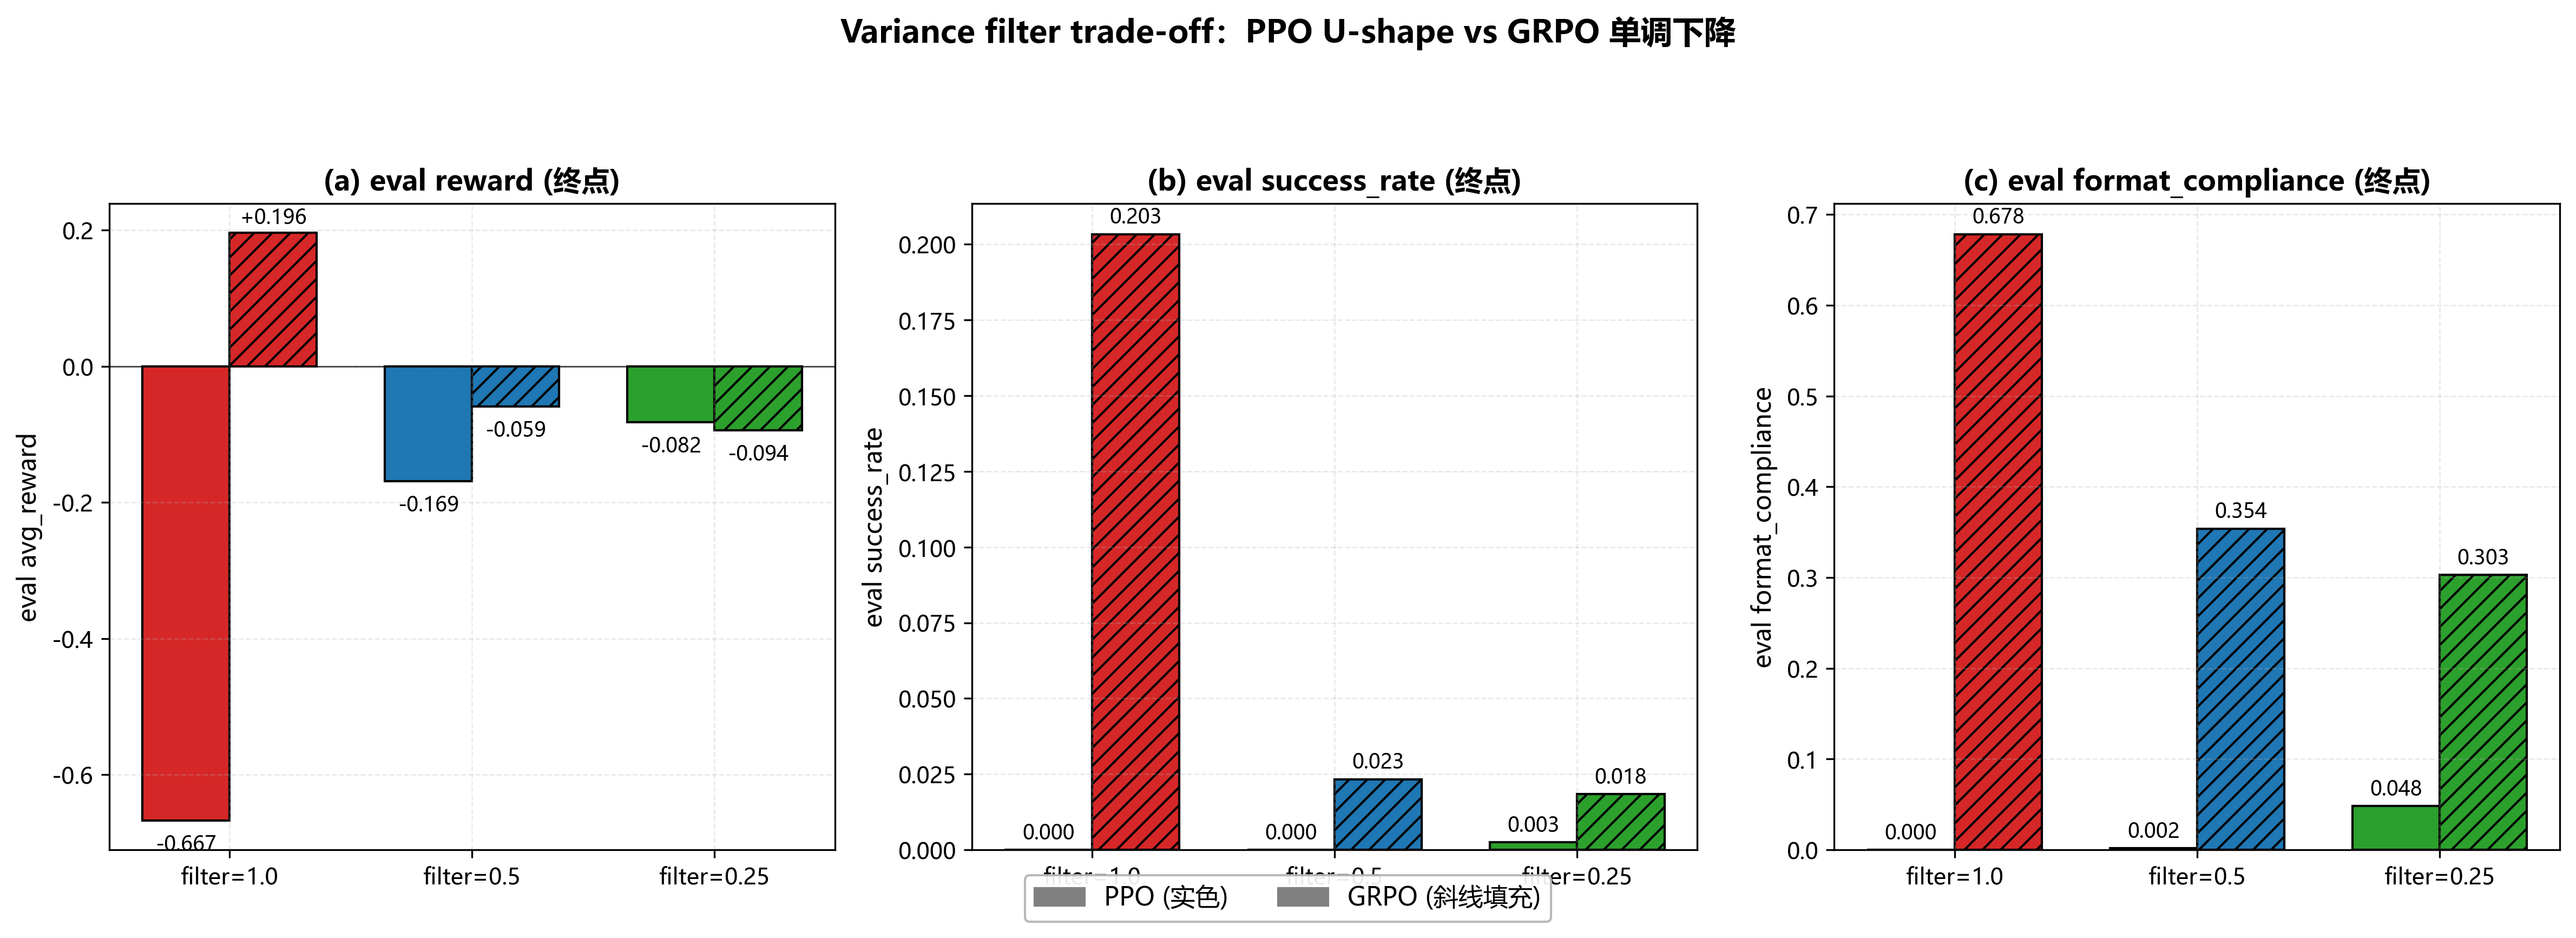
\includegraphics[width=\linewidth]{figures/fig06_filter_tradeoff_bar.png}
\caption{Final-reward view of the filter trade-off. PPO and GRPO respond to filtering in opposite directions.}
\label{fig:tradeoff}
\end{figure}

\subsection{PPO Collapse Is Format Collapse, Not Classic Echo Trap}

The vanilla PPO failure does not match RAGEN's classic echo-trap signature. RAGEN echo trap is characterized by repeated invalid modes and decreasing entropy. Here, PPO vanilla enters a format collapse: reward falls, format compliance reaches zero, KL spikes sharply, and entropy increases rather than decreases.

\begin{figure*}[t]
\centering

\includegraphics[width=\figw]{figures/fig07_train_entropy_6groups.png}
\caption{Training entropy. PPO vanilla moves toward higher entropy during collapse, while GRPO vanilla decreases entropy while improving reward and format compliance.}
\label{fig:entropy}
\end{figure*}

\begin{figure*}[t]
\centering

\includegraphics[width=\figw]{figures/fig08_train_kl_grad_6groups.png}
\caption{KL penalty and pre-clip gradient norm. PPO runs have much larger gradient norms than GRPO runs, and PPO vanilla shows a large KL spike near the collapse boundary.}
\label{fig:klgrad}
\end{figure*}

Figures~\ref{fig:entropy} and~\ref{fig:klgrad} make the distinction visible. PPO vanilla reaches the highest entropy among the six runs, while format compliance falls to zero. The run also shows an extreme KL spike near the collapse boundary. This points to a failure mode in which the policy moves away from the reference model into high-entropy malformed output, rather than converging to a deterministic repeated phrase.

\subsection{Filter Ratio 0.25 Degenerates to Single-Step Updates}

With \(P=8\), \(K=16\), and effective mini-batch size 32, the number of gradient steps per training iteration is
\begin{equation}
n_{\mathrm{grad}} =
\left\lceil \frac{r \cdot P \cdot K}{32} \right\rceil.
\end{equation}
Thus ratios \(1.0\), \(0.5\), and \(0.25\) produce 4, 2, and 1 gradient steps respectively.

\begin{figure}[t]
\centering
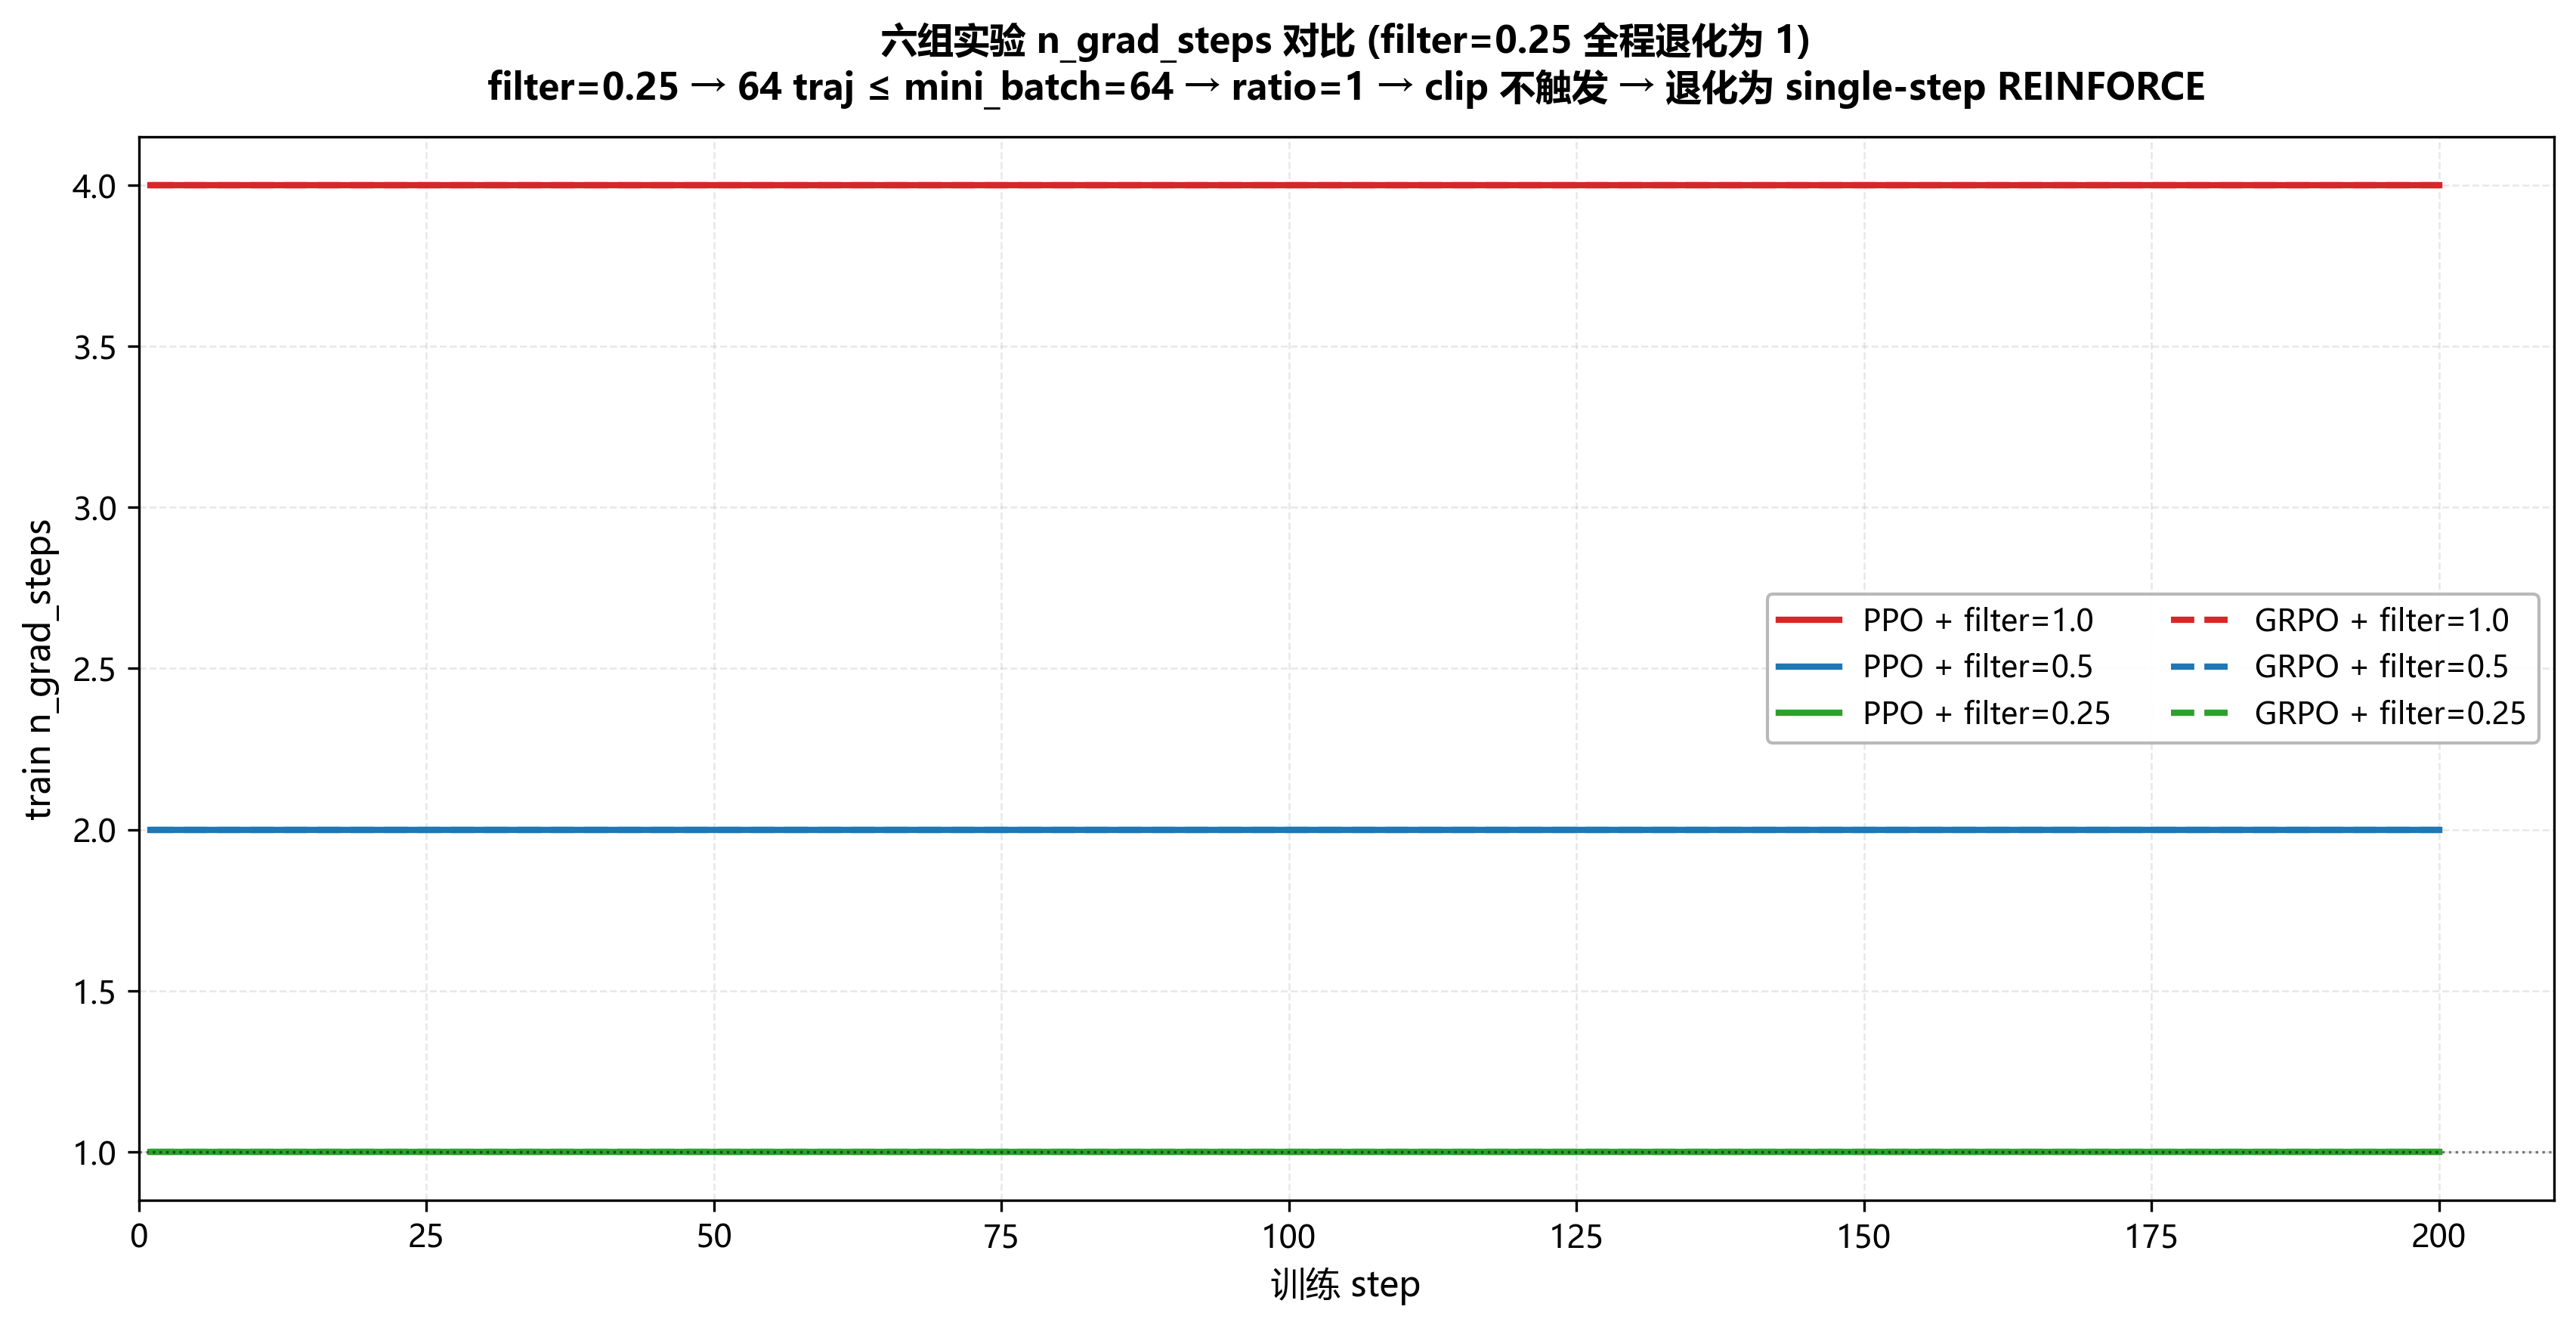
\includegraphics[width=\linewidth]{figures/fig09_n_grad_steps_6groups.png}
\caption{The number of optimizer steps is determined by filter ratio under the fixed effective mini-batch size. Ratio 0.25 gives exactly one update step.}
\label{fig:ngrad}
\end{figure}

At ratio 0.25, the filtered buffer contains exactly 32 trajectories, equal to one mini-batch. With one epoch, the first and only update sees current log probabilities equal to old log probabilities, so the PPO ratio is one, clipping never activates, and approximate KL is zero. This degeneration affects both PPO and GRPO because GRPO reuses the PPO-style clipped surrogate. The stability of the 0.25 runs is therefore better interpreted as conservative single-step REINFORCE-like behavior~\citep{williams1992reinforce}, not as proof that aggressive variance filtering is intrinsically superior.

\subsection{GRPO Reverses the StarPO-S Pattern}

\begin{figure*}[t]
\centering
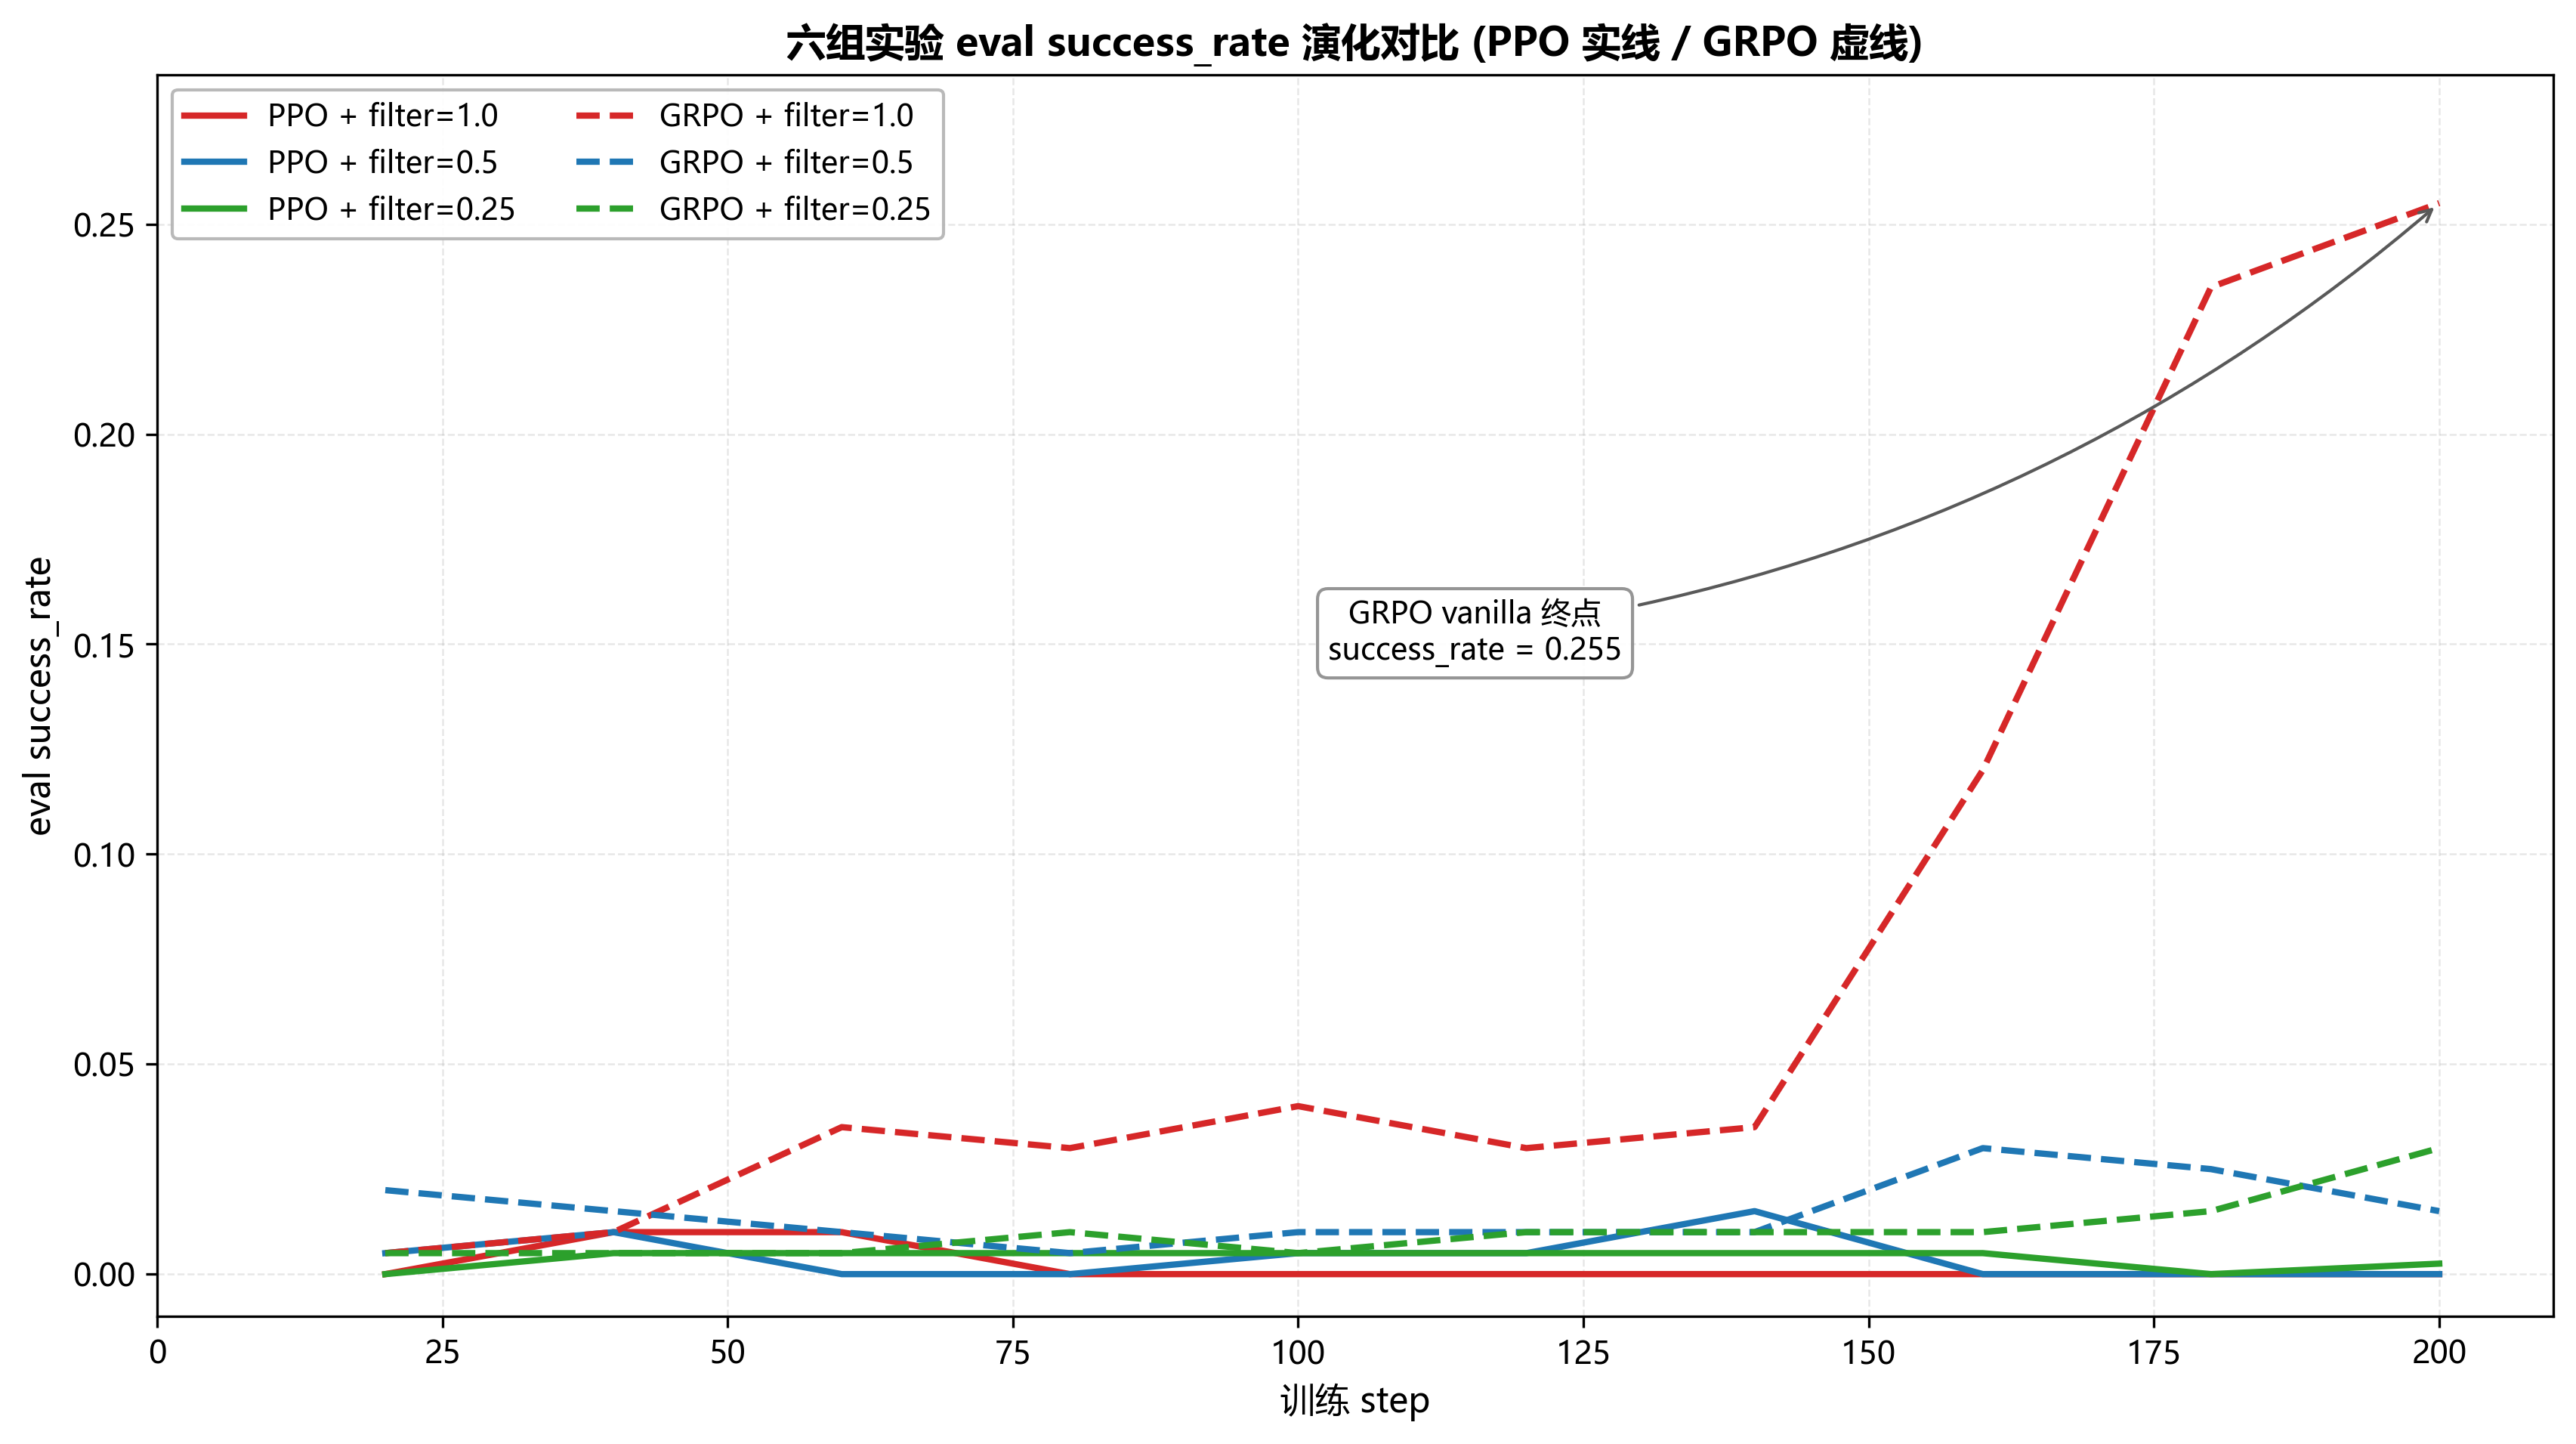
\includegraphics[width=\figw]{figures/fig02_eval_success_6groups.png}
\caption{Evaluation success rate. GRPO vanilla is the only run with substantial task success at the end of training.}
\label{fig:success}
\end{figure*}

\begin{figure*}[t]
\centering

\includegraphics[width=\figw]{figures/fig03_eval_format_6groups.png}
\caption{Format compliance. GRPO vanilla rises to approximately 0.81, while PPO variants and filtered GRPO variants remain much weaker.}
\label{fig:format}
\end{figure*}

The GRPO runs are the main extension beyond a straightforward reproduction. GRPO vanilla is the only run that reaches positive reward, non-trivial success, and high format compliance. Figures~\ref{fig:success} and~\ref{fig:format} show that its reward improvement is not a metric artifact: the agent both solves the task more often and preserves the required output structure.

\begin{figure*}[t]
\centering

\includegraphics[width=\figw]{figures/fig04_eval_panel_5metrics.png}
\caption{Five evaluation metrics. GRPO vanilla is strongest or tied strongest across the main evaluation dimensions.}
\label{fig:panel}
\end{figure*}

At the claim level, the GRPO column is opposite to the PPO column:
\begin{itemize}
\item Vanilla GRPO is not unstable; it is the strongest run.
\item Filtering does not repair vanilla GRPO; it makes GRPO worse.
\item The best GRPO filter ratio is 1.0, not 0.5.
\end{itemize}

\subsection{Why Filtering Helps PPO but Hurts GRPO}

The mechanism has three layers.

\paragraph{Critic-data amplification exists only in PPO.}
For PPO, high-variance prompts provide useful value-function targets: the same prompt can produce trajectories with different returns, so the critic receives informative state-return contrasts. A better critic improves advantage estimates and stabilizes the actor update. In this sense, variance filtering acts as data selection for the critic.

GRPO has no critic. Its advantage is a within-group z-score. Once the group has nonzero reward variation, scaling the reward spread does not proportionally scale the advantage. Filtering high-variance groups therefore does not provide the same signal amplification; it mostly removes samples.

\paragraph{Sample removal is more costly in GRPO.}
For PPO, the benefit of cleaner critic data can partially offset the harm of fewer samples, producing a sweet spot. For GRPO, the benefit side is much weaker. Reducing samples increases gradient variance and reduces the number of update mini-batches without providing a compensating critic-training improvement.

\paragraph{The 0.25 boundary is shared.}
Both algorithms degenerate at ratio 0.25 under the single-GPU mini-batch configuration. This explains why both aggressive-filter runs appear stable but stagnant.

\subsection{Echo-Trap Proxy Needs Reward and Format}

\begin{figure*}[t]
\centering
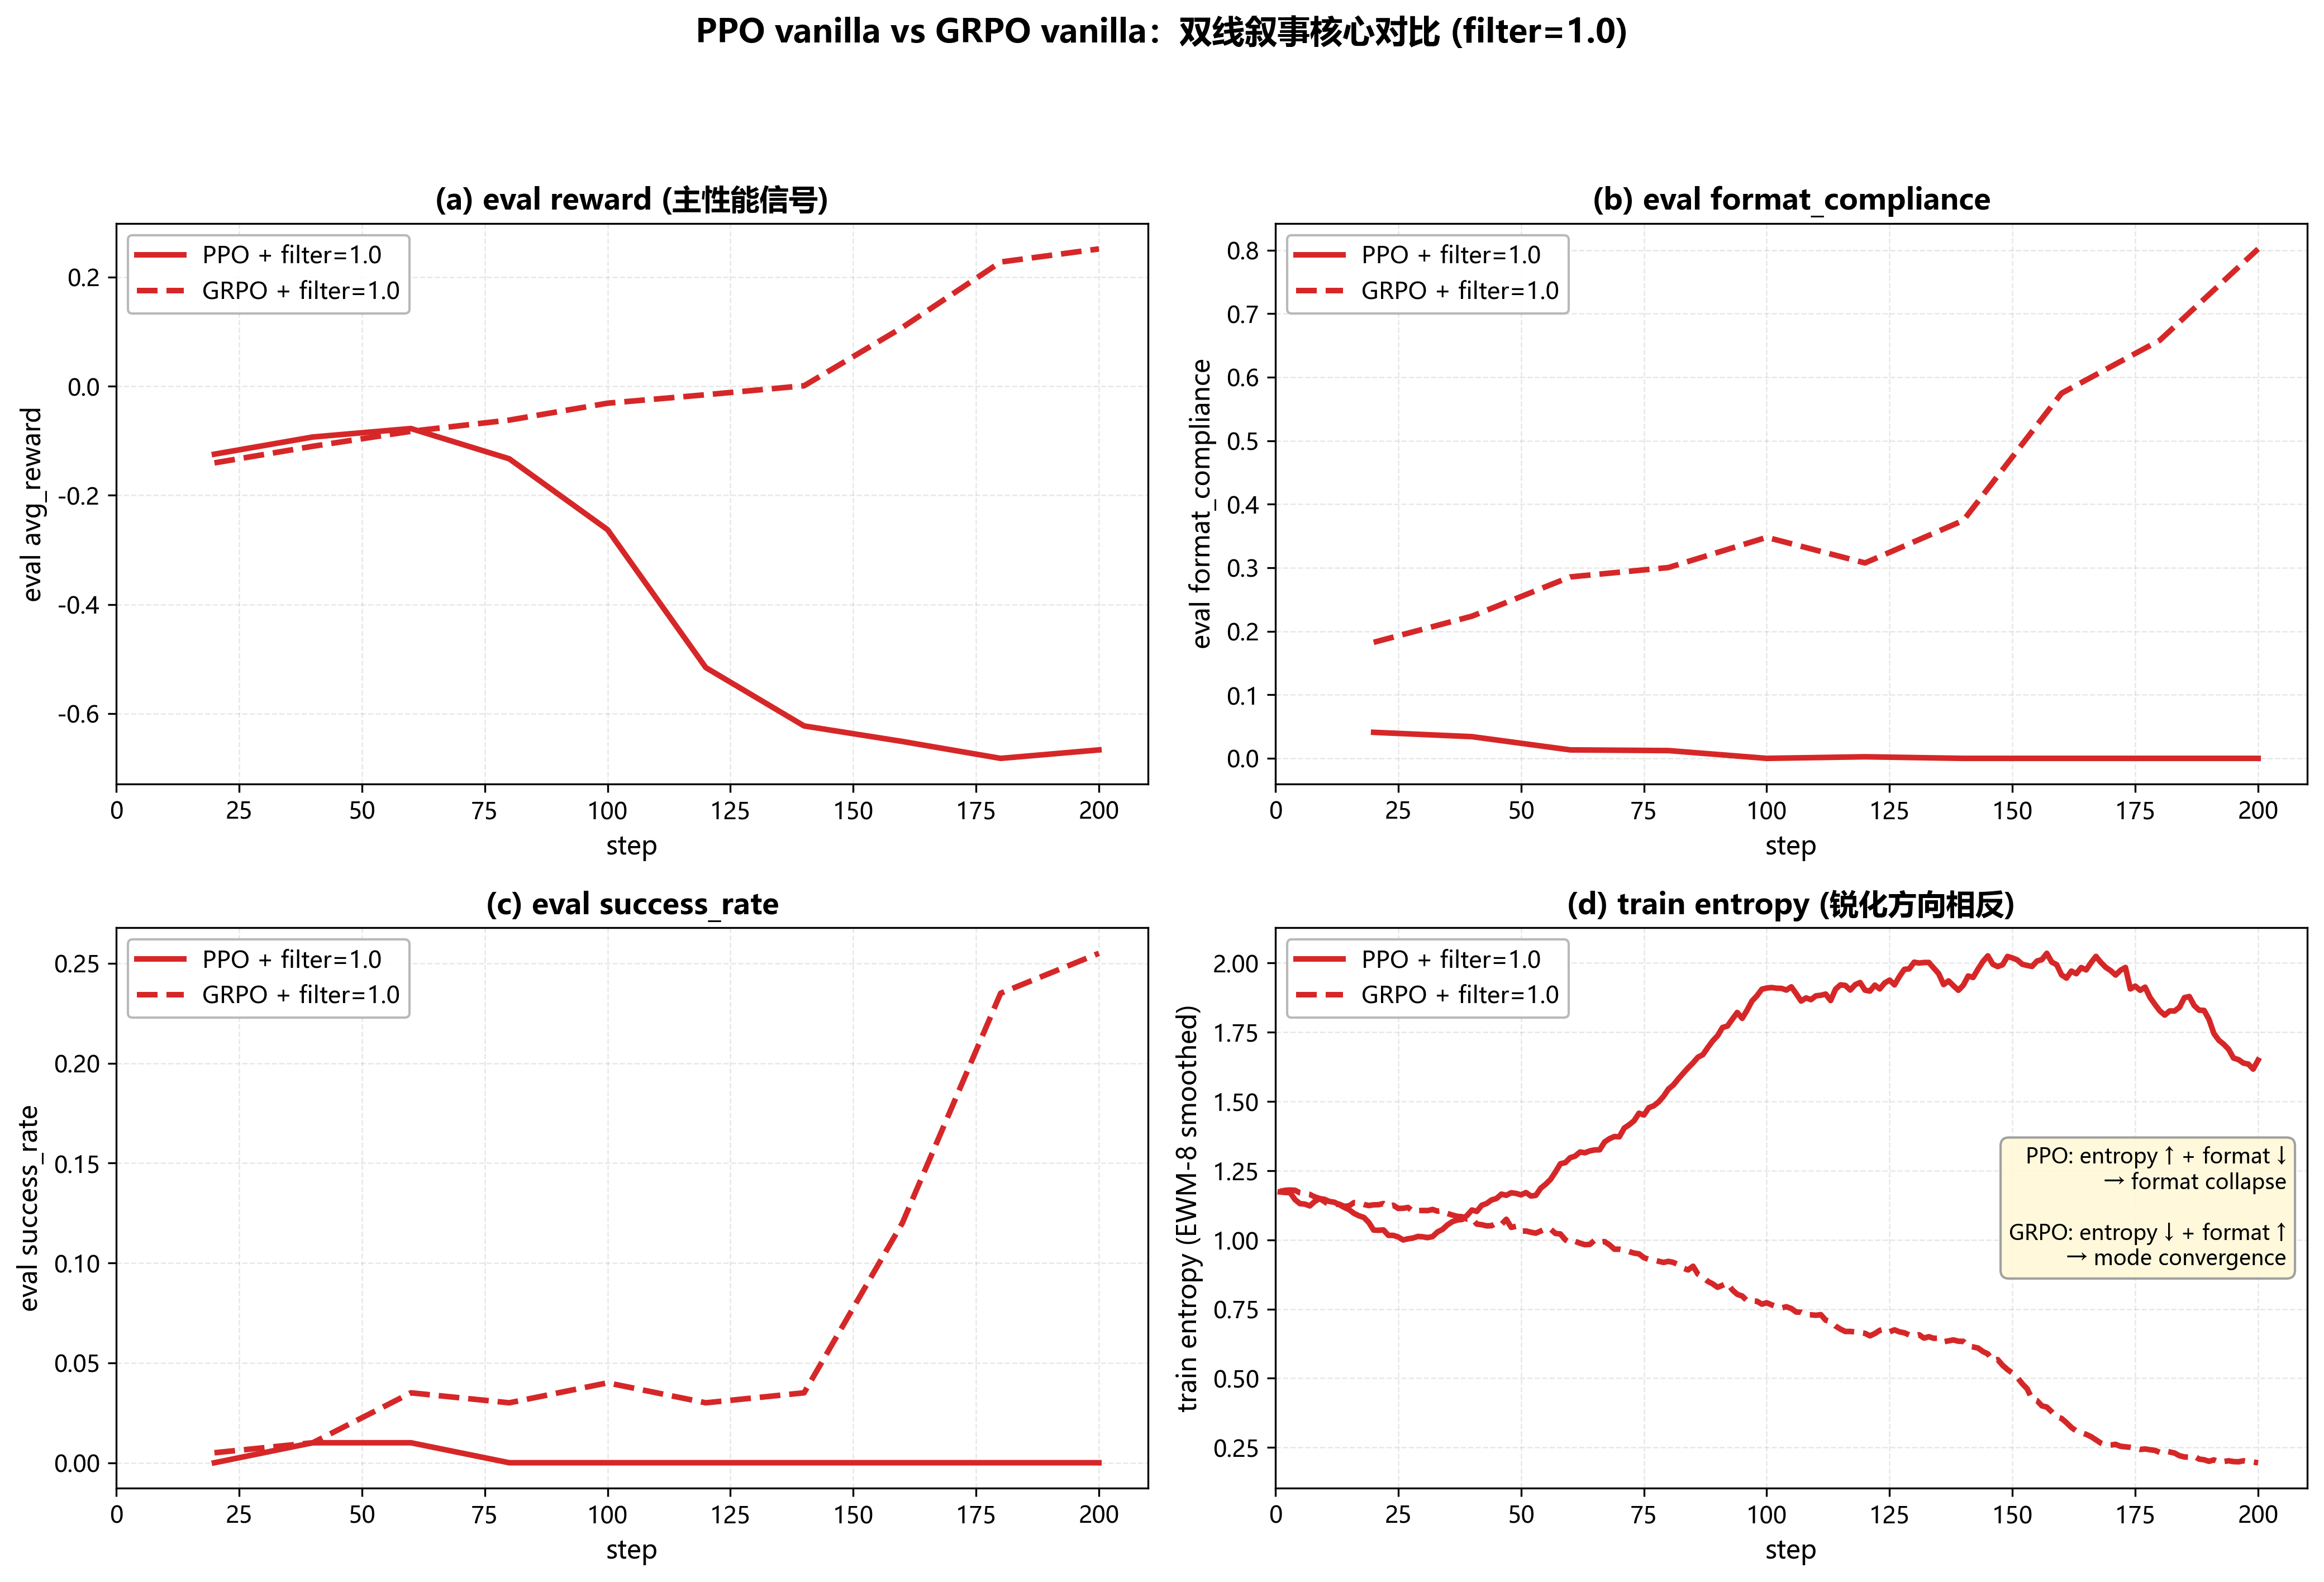
\includegraphics[width=\figw]{figures/fig05_ppo_vs_grpo_vanilla.png}
\caption{Head-to-head comparison of PPO vanilla and GRPO vanilla. The two runs move in opposite directions across reward, entropy, format compliance, and success rate.}
\label{fig:headtohead}
\end{figure*}

\begin{figure*}[t]
\centering
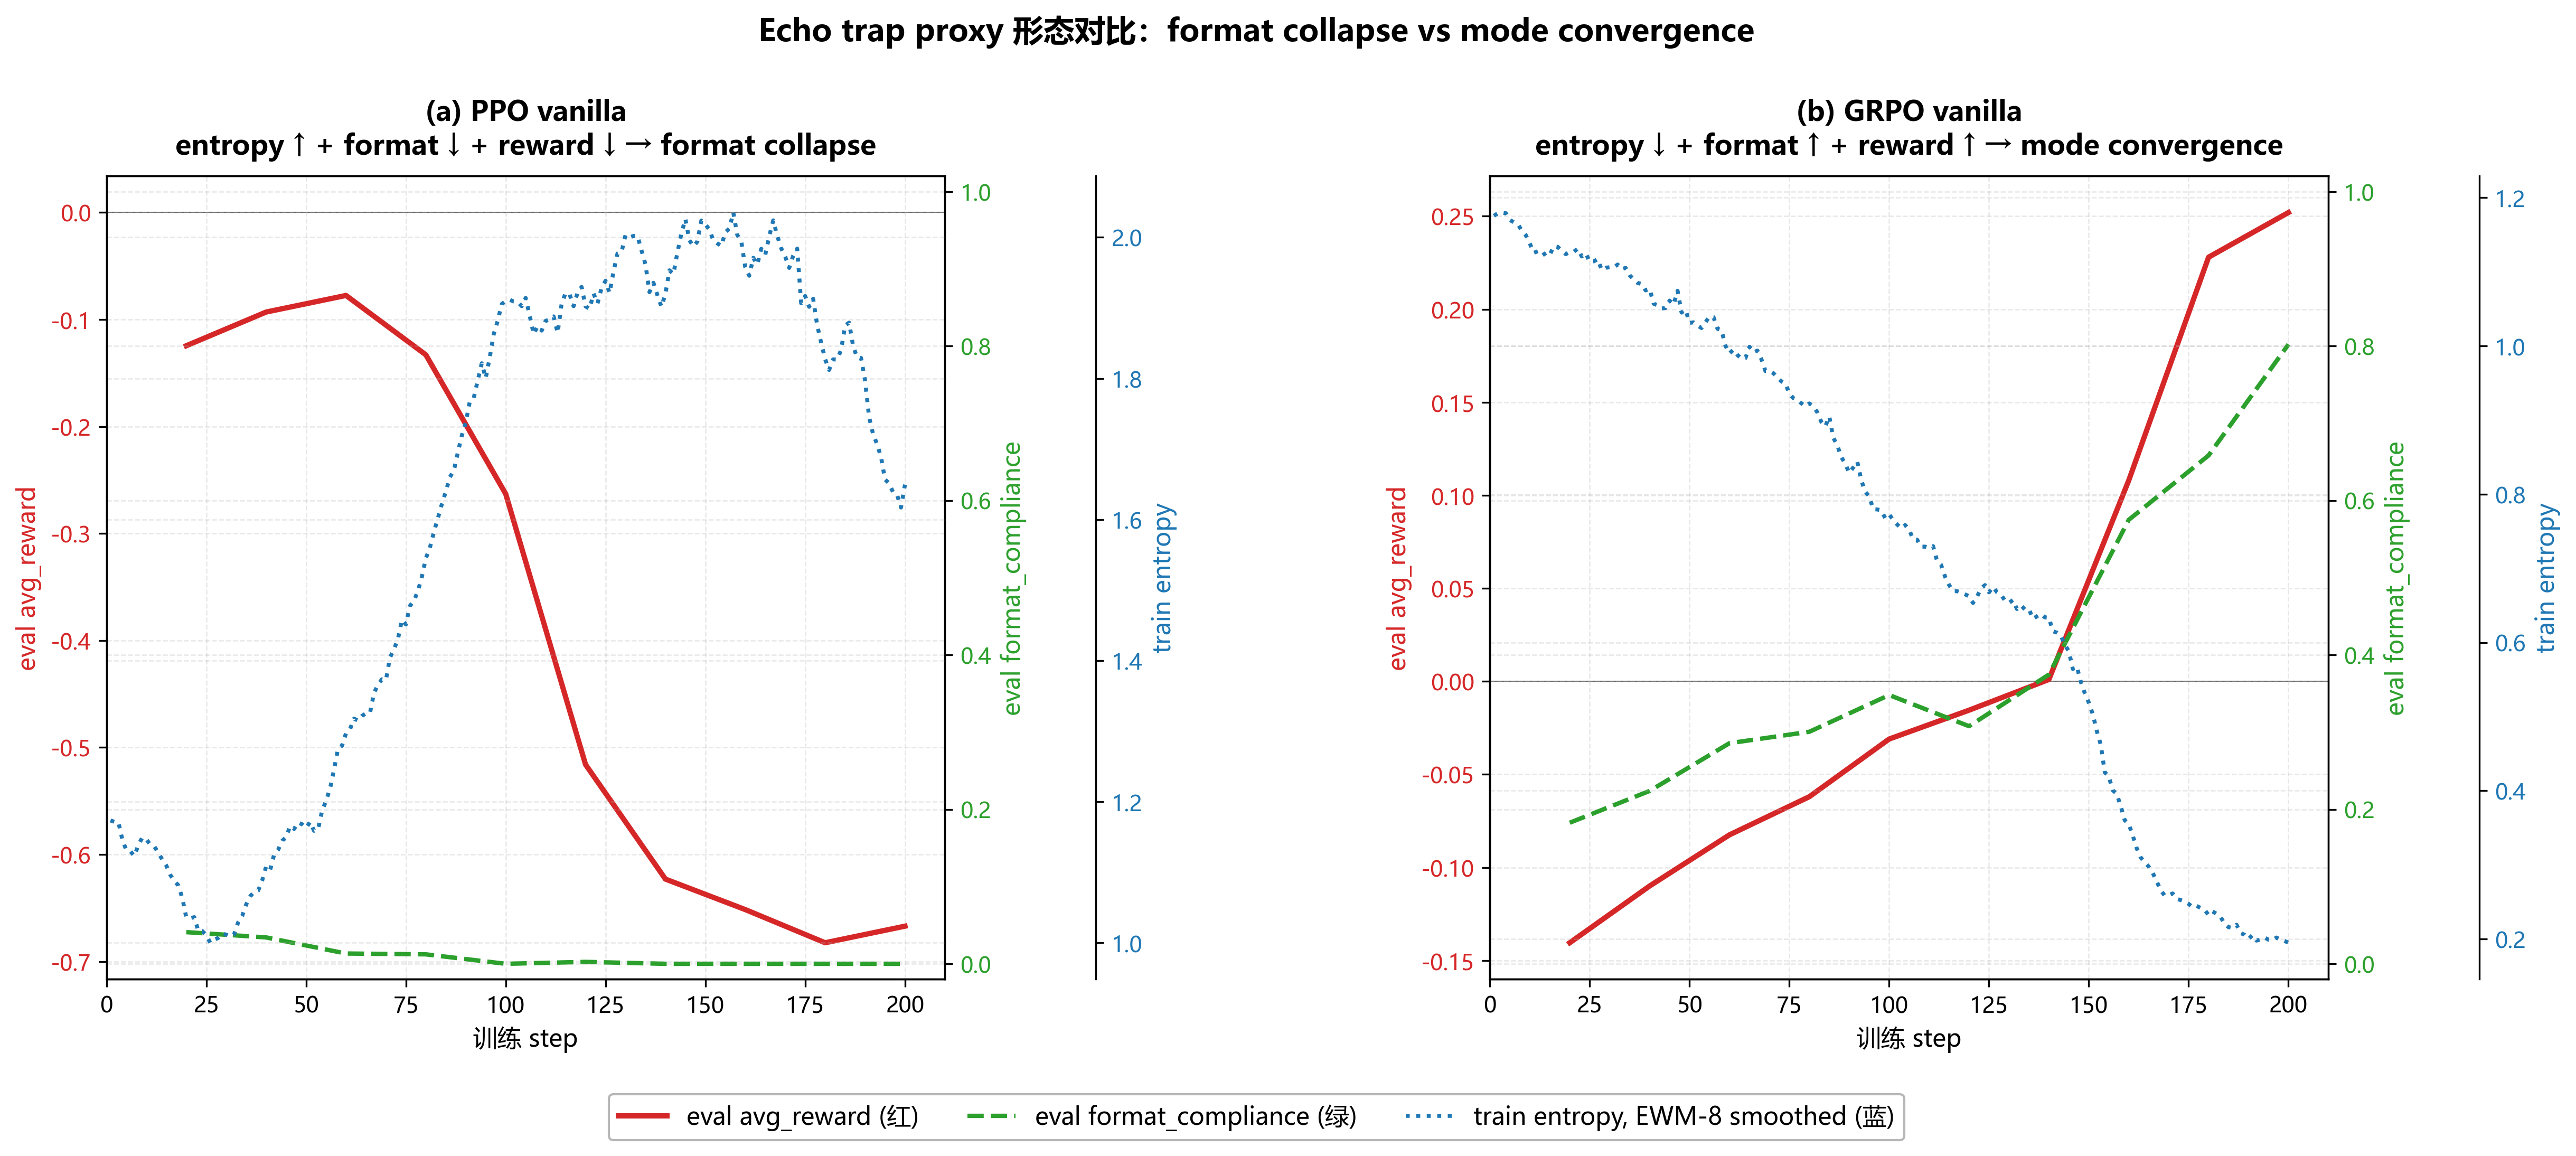
\includegraphics[width=\figw]{figures/fig10_echo_trap_proxy.png}
\caption{Joint echo-trap proxy. Entropy alone is ambiguous; reward and format compliance separate unhealthy collapse from healthy mode convergence.}
\label{fig:echoproxy}
\end{figure*}

Entropy decrease alone is not enough to diagnose echo trap. Figure~\ref{fig:headtohead} shows that PPO vanilla and GRPO vanilla are opposite across all four key dimensions. PPO vanilla has reward down, entropy up, format down, and success zero. GRPO vanilla has reward up, entropy down, format up, and success up.

Figure~\ref{fig:echoproxy} motivates a stronger diagnostic: echo trap should be treated as a joint pattern involving entropy, reward, and format compliance. Low entropy with rising reward and rising format compliance is healthy mode convergence. Low entropy with stagnant or falling reward is a candidate echo trap. High entropy with format collapse is a different failure mode.

\subsection{Quantization Noise and Algorithm Scale}

The PPO runs have pre-clip gradient norms in the hundreds or thousands, while GRPO remains around \(0.05\)--\(0.16\). This is consistent with the different advantage scales: PPO's bi-level GAE can produce larger token-level weights, while GRPO z-scores are naturally bounded to a small range.

Because AdamW8bit introduces block-wise optimizer-state quantization noise~\citep{dettmers2022optimizers}, PPO's larger update scale and critic coupling may be more sensitive to numerical drift. GRPO provides a useful controlled contrast: it uses the same hardware concessions and optimizer family but avoids the critic and uses smaller advantages. Its strong vanilla performance suggests that part of PPO's collapse is an algorithm-by-hardware interaction rather than a pure reproduction of RAGEN's original echo-trap dynamics.
